\begin{center}
    \section*{\LARGE Anexos}    
\end{center}
\addcontentsline{toc}{chapter}{Anexos}

\subsection*{Anexo 1: Código fuente del sistema}\label{Anexo1}

\begin{flushleft}
    \begin{figure}[H]
        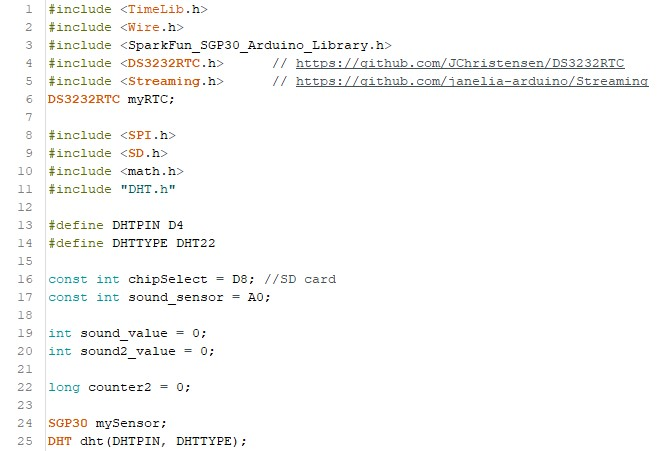
\includegraphics{imagenes/codigo1.jpg}
        \caption*{Segmento 1}
    \end{figure}
    
    \begin{figure}[H]
        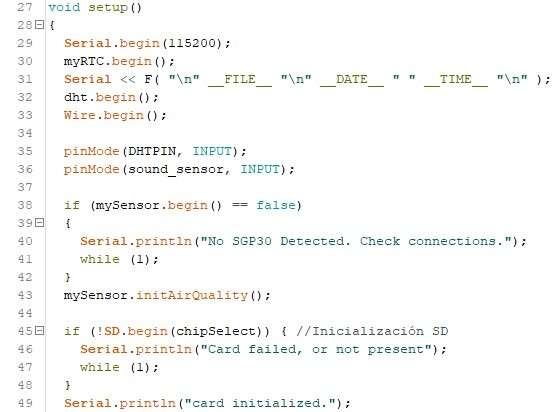
\includegraphics{imagenes/codigo2.jpg}
        \caption*{Segmento 2}
    \end{figure}
    
    \begin{figure}[H]
        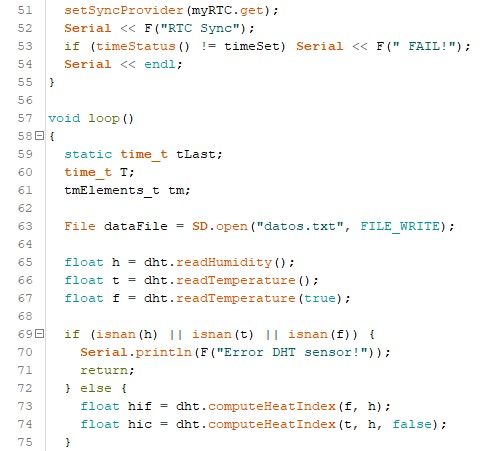
\includegraphics{imagenes/codigo3.jpg}
        \caption*{Segmento 3}
    \end{figure}
    
    \begin{figure}[H]
        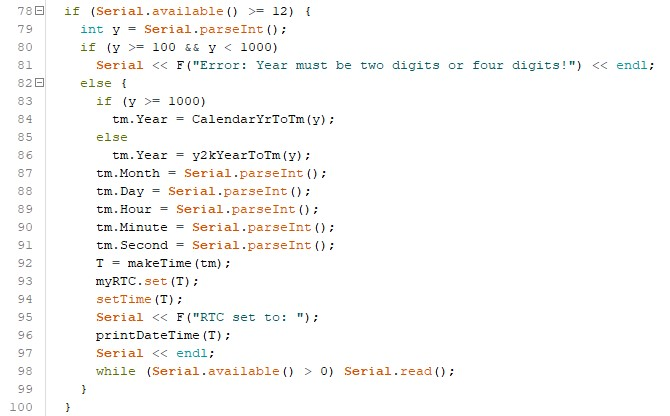
\includegraphics{imagenes/codigo4.jpg}
        \caption*{Segmento 4}
    \end{figure}
    
    \begin{figure}[H]
        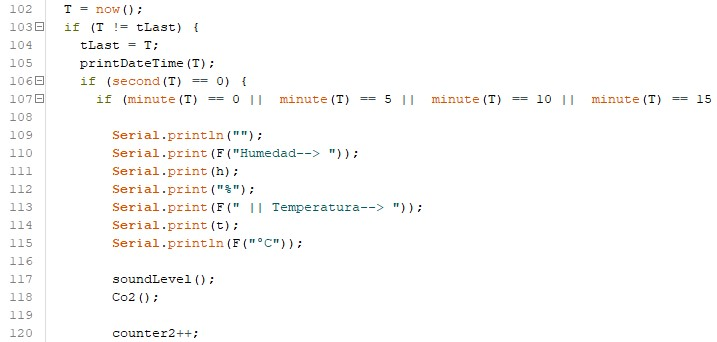
\includegraphics{imagenes/codigo5.jpg}
        \caption*{Segmento 5}
    \end{figure}
    
    \begin{figure}[H]
        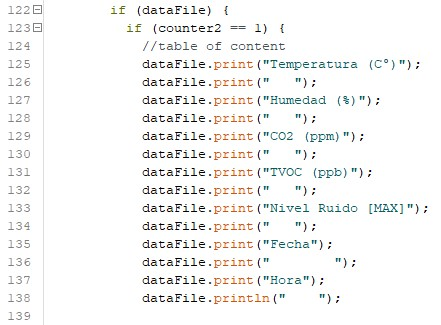
\includegraphics{imagenes/codigo6.jpg}
        \caption*{Segmento 6}
    \end{figure}

    \begin{figure}[H]
        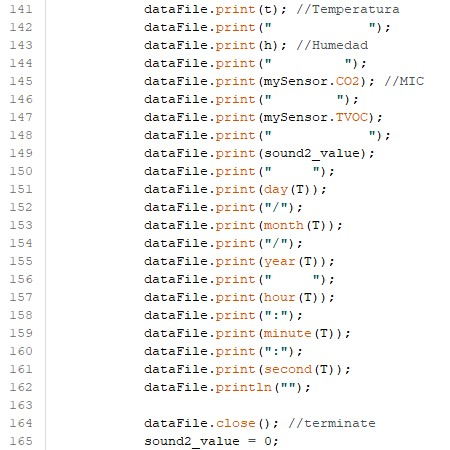
\includegraphics{imagenes/codigo7.jpg}
        \caption*{Segmento 7}
    \end{figure}

    \begin{figure}[H]
        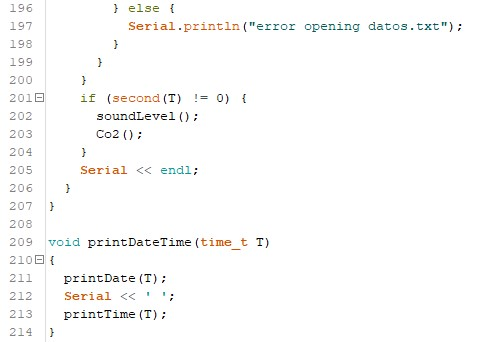
\includegraphics{imagenes/codigo8.jpg}
        \caption*{Segmento 8}
    \end{figure}

    \begin{figure}[H]
        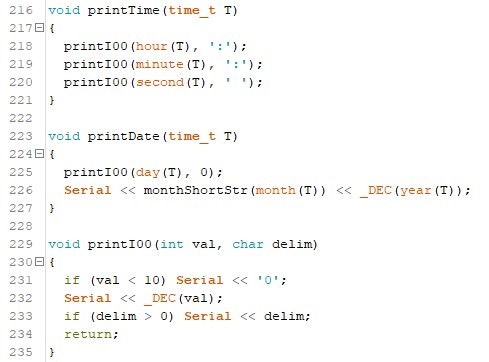
\includegraphics{imagenes/codigo9.jpg}
        \caption*{Segmento 9}
    \end{figure}

    \begin{figure}[H]
        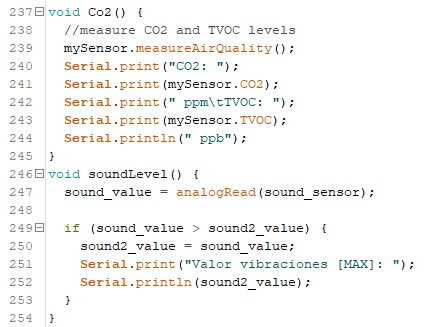
\includegraphics{imagenes/codigo10.jpg}
        \caption*{Segmento 10}
    \end{figure}
\end{flushleft}

\subsection*{Anexo 2: Placa de circuito impreso del nuevo prototipo de Nodo para las vitrinas}\label{Anexo2}

\begin{figure}[H]
    \centering
    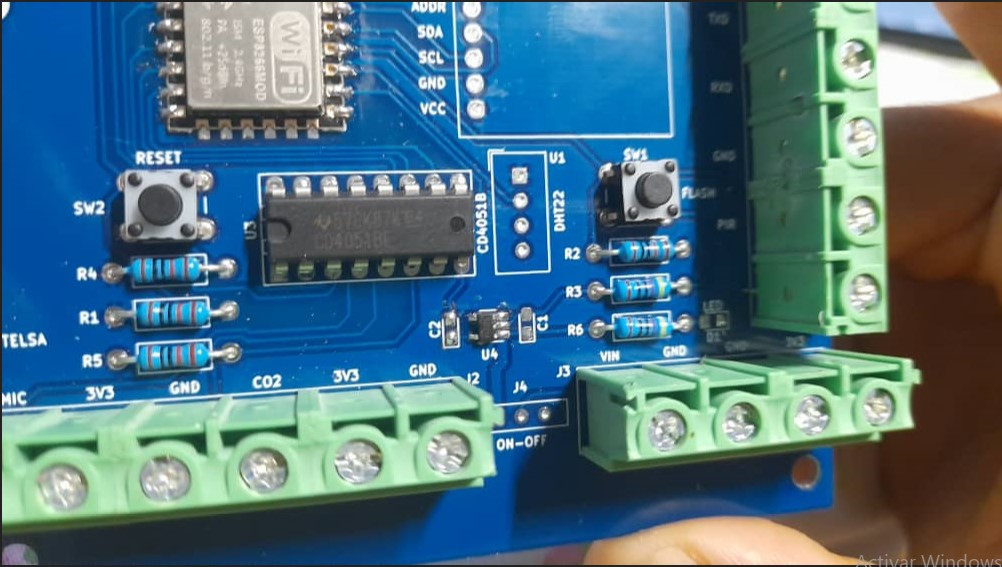
\includegraphics[width = 14.5cm, height = 11cm]{imagenes/pcb placa.jpg}
    \caption*{PCB Nodo Vitrinas}
\end{figure}


